\documentclass[11pt]{article}
\usepackage[utf8]{inputenc}

% add LaTeX packages to use here
\usepackage{amsmath}
\usepackage{amssymb}
\usepackage{amsfonts}
\usepackage{amsthm}
\usepackage{fancyhdr}
\usepackage{lastpage}
\usepackage{enumitem}
\usepackage{framed}
\usepackage[most]{tcolorbox}
\usepackage{geometry}
\usepackage{graphicx}

 % set dimensions for page layout
\geometry
{
 left=5em,
 right=5em,
 bottom=5em,
 top=6em,
 headheight=110pt,
 showframe=false
}

\setlist[itemize]{leftmargin=*} % prevents indenting of itemize

% abbreviations for some common math symbols
\newcommand{\Rset}{\hbox{$\mathbb R$}}
\newcommand{\Nset}{\hbox{$\mathbb N$}}
\newcommand{\Pset}{\hbox{$\mathbb{N}^{+}$}}
\newcommand{\Zset}{\hbox{$\mathbb N$}}
\newcommand{\Qset}{\hbox{$\mathbb Q$}}

% theorem style
\newtheoremstyle{thmstyle}% name of the style to be used
  {0pt}% measure of space to leave above the theorem. E.g.: 3pt
  {0pt}% measure of space to leave below the theorem. E.g.: 3pt
  {}% name of font to use in the body of the theorem
  {}% measure of space to indent
  {\bfseries}% name of head font
  {.}% punctuation between head and body
  { }% space after theorem head; " " = normal inter-word space
  {}% Manually specify head

% theorem environment instance
\theoremstyle{thmstyle}
\newtheorem{theorem}{Theorem}

% shaded and framed solution environment 
\makeatletter
\newenvironment{shadedSolutionBox}
  {\setlength{\OuterFrameSep}{0in}%
  \definecolor{shadecolor}{gray}{.8}% shading of shaded solution box
  \bigskip%
  \@nameuse{shaded*}\par\noindent\ignorespaces \textit{Solution}.}
  {\hspace{\stretch{1}}\rule{1.5ex}{1.5ex}% adds filled box 
  \@nameuse{endshaded*}%
  \bigskip}
\makeatother

% shaded and framed theorem environment 
\makeatletter
\newenvironment{thm}
  {\setlength{\OuterFrameSep}{0in}%
  \definecolor{shadecolor}{gray}{1}% shading of shaded Theorem box
  \@nameuse{snugshade*}\par\noindent\ignorespaces%
   \@nameuse{theorem}}
  {\hspace{\stretch{1}}\scalebox{1.5}{\hbox{$\triangleleft$}}% adds triangle shape
  \@nameuse{endtheorem}%
  \@nameuse{endsnugshade*}%
  }
\makeatother

% header and footer elements of every page except the first.
\pagestyle{fancy}
\fancyfoot[L]{\textsc{CISC {\small\selectfont 3230}} }
\fancyhead[R]{{\small\selectfont\textsc{\studentLastName}}}
\fancyfoot[C]{{\small\selectfont\assignmentName}}
\fancyfoot[R]{{\small\selectfont\thepage\ of \pageref{LastPage}}}
\renewcommand{\headrulewidth}{0.8pt}
\renewcommand{\footrulewidth}{0.4pt}

% hline with variable thickness
\makeatletter
\def\thickhline{%
  \noalign{\ifnum0=`}\fi\hrule \@height \thickarrayrulewidth \futurelet
   \reserved@a\@xthickhline}
\def\@xthickhline{\ifx\reserved@a\thickhline
               \vskip\doublerulesep
               \vskip-\thickarrayrulewidth
             \fi
      \ifnum0=`{\fi}}
\makeatother

% length instance for \thickhline
\newlength{\thickarrayrulewidth} 
\setlength{\thickarrayrulewidth}{.8pt}

% header and footer for first page
\fancypagestyle{firstpage}
{
\fancyhf{}
\renewcommand{\footrulewidth}{0.4pt}
\renewcommand{\headrulewidth}{0pt}
\fancyhead[C]{%
\begin{tabular*}{\textwidth}{@{\extracolsep{\fill}}@{}l @{} c @{} r @{} }
{\small\selectfont\courseName}&{\normalsize\selectfont\assignmentName}&{\small\selectfont\studentFirstName\ \studentLastName}\\
\thickhline
&&{\scriptsize\selectfont\collaboratorNames}
\end{tabular*}%
}
\fancyfoot[R]{{\small\selectfont\thepage\ of \pageref{LastPage}}}
\fancyfoot[L]{{\footnotesize\selectfont\pdfcreationdate}}
}

\newcommand{\courseName}{Theoretical Computer Science} % course name

% your first name, your last name, and the assignment name
\newcommand{\studentLastName}{Nikabadze} % your last name
\newcommand{\studentFirstName}{Luka} % your first name (and middle name, if applicable)
\newcommand{\assignmentName}{Homework 1 part 1} % the assignment name
\newcommand{\collaboratorNames}{[First Name Initial]. Last Name} % if you worked with anyone to complete any part of the assignment, include the initial of the first name (and middle name, if applicable) and full last name of each of your collaborators, separated by commas (e.g., if you worked with Arthur Paul Pedersen and Sandra Lee, include "A.P. Pedersen, S. Lee")




\begin{document} % marks the beginning of the document

\thispagestyle{firstpage} % institutes page style for first page

\setlength{\abovedisplayskip}{20pt} % space above math in align* environment
\setlength{\belowdisplayskip}{20pt} % space below math in align* environment



% marks the beginning of the document body


\begin{itemize}\setlength{\itemsep}{1em} % \itemsep is the spacing between items in environment
\item[4.e]  Consider the Language L = {w|w Start and an a and has at most one b } The language l is the intersection of two simpler languages $L_1$ and $L_2$. no $L_1$= { w|w starts with a} and $L_1$ = {w|w has at most one b} Let M be the DFA and $M_1$ and $M_2$ be and DFAs that recognizes $L_1$ and $L_2$ . 

• below is given DFA of $M_1$
\documentclass[12pt]{article} \usepackage{tikz}
\begin{document}
\begin{center} 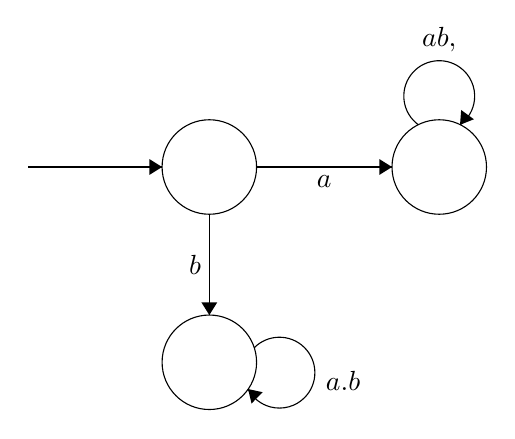
\begin{tikzpicture}[scale=0.2] \tikzstyle{every node}+=[inner sep=0pt] \draw [black] (44.3,-16) circle (3); \draw [black] (29.7,-16) circle (3); \draw [black] (29.7,-28.4) circle (3); \draw [black] (42.977,-13.32) arc (234:-54:2.25); \draw (44.3,-8.75) node [above] {$ab,$}; \fill [black] (45.62,-13.32) -- (46.5,-12.97) -- (45.69,-12.38); \draw [black] (32.7,-16) -- (41.3,-16); \fill [black] (41.3,-16) -- (40.5,-15.5) -- (40.5,-16.5); \draw (37,-16.5) node [below] {$a$}; \draw [black] (18.2,-16) -- (26.7,-16); \fill [black] (26.7,-16) -- (25.9,-15.5) -- (25.9,-16.5); \draw [black] (29.7,-19) -- (29.7,-25.4); \fill [black] (29.7,-25.4) -- (30.2,-24.6) -- (29.2,-24.6); \draw (29.2,-22.2) node [left] {$b$}; \draw [black] (32.545,-27.484) arc (135.57303:-152.42697:2.25); \draw (37.07,-29.57) node [right] {$a.b$}; \fill [black] (32.16,-30.1) -- (32.38,-31.02) -- (33.08,-30.3); \end{tikzpicture} \end{center}

• below is given DFA of $M_2$


\begin{document}
\begin{center} 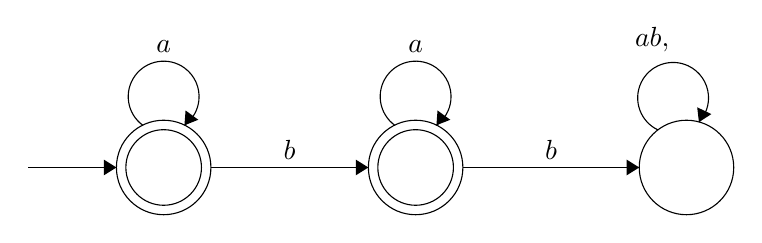
\begin{tikzpicture}[scale=0.2] \tikzstyle{every node}+=[inner sep=0pt] \draw [black] (18.7,-17.6) circle (3); \draw [black] (18.7,-17.6) circle (2.4); \draw [black] (34.7,-17.6) circle (3); \draw [black] (34.7,-17.6) circle (2.4); \draw [black] (51.9,-17.6) circle (3); \draw [black] (10.1,-17.6) -- (15.7,-17.6); \fill [black] (15.7,-17.6) -- (14.9,-17.1) -- (14.9,-18.1); \draw [black] (21.7,-17.6) -- (31.7,-17.6); \fill [black] (31.7,-17.6) -- (30.9,-17.1) -- (30.9,-18.1); \draw (26.7,-17.1) node [above] {$b$}; \draw [black] (17.377,-14.92) arc (234:-54:2.25); \draw (18.7,-10.35) node [above] {$a$}; \fill [black] (20.02,-14.92) -- (20.9,-14.57) -- (20.09,-13.98); \draw [black] (33.377,-14.92) arc (234:-54:2.25); \draw (34.7,-10.35) node [above] {$a$}; \fill [black] (36.02,-14.92) -- (36.9,-14.57) -- (36.09,-13.98); \draw [black] (50.095,-15.218) arc (244.88553:-43.11447:2.25); \draw (49.72,-10.32) node [above] {$ab,$}; \fill [black] (52.69,-14.72) -- (53.48,-14.21) -- (52.58,-13.78); \draw [black] (37.7,-17.6) -- (48.9,-17.6); \fill [black] (48.9,-17.6) -- (48.1,-17.1) -- (48.1,-18.1); \draw (43.3,-17.1) node [above] {$b$}; \end{tikzpicture} \end{center}



\item[4.f] Consider the language L = { w|w has an odd number of A's and ends with b}. the language L is the intersection of two simpler languages say $L_1$ and $L_2$. Now $L_1$ = {w|w has an odd number of a's } and $L_2$ = {w|w end with a b} let M be be DFA that recognizes L and $M_1$ and $M_2$ be the DFA that recognizes $L_1$ and $L_2$

• below is given DFA of $M_1$
\usepackage{tikz}

\begin{document}

\begin{center}
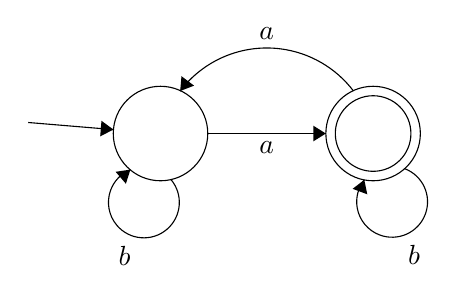
\begin{tikzpicture}[scale=0.2]
\tikzstyle{every node}+=[inner sep=0pt]
\draw [black] (32.8,-17.8) circle (3);
\draw [black] (46.3,-17.8) circle (3);
\draw [black] (46.3,-17.8) circle (2.4);
\draw [black] (35.8,-17.8) -- (43.3,-17.8);
\fill [black] (43.3,-17.8) -- (42.5,-17.3) -- (42.5,-18.3);
\draw (39.55,-18.3) node [below] {$a$};
\draw [black] (34.047,-15.098) arc (142.78436:37.21564:6.91);
\fill [black] (34.05,-15.1) -- (34.93,-14.76) -- (34.13,-14.16);
\draw (39.55,-11.87) node [above] {$a$};
\draw [black] (24.4,-17.1) -- (29.81,-17.55);
\fill [black] (29.81,-17.55) -- (29.05,-16.99) -- (28.97,-17.98);
\draw [black] (33.457,-20.715) arc (40.42334:-247.57666:2.25);
\draw (30.52,-24.93) node [below] {$b$};
\fill [black] (30.89,-20.09) -- (29.95,-20.23) -- (30.6,-20.99);
\draw [black] (48.293,-20.027) arc (69.55109:-218.44891:2.25);
\draw (48.9,-24.86) node [below] {$b$};
\fill [black] (45.74,-20.74) -- (45,-21.31) -- (45.93,-21.66);
\end{tikzpicture}
\end{center}

• below is given DFA of $M_2$



\begin{document}

\begin{center}
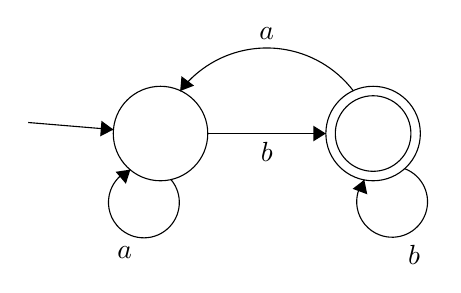
\begin{tikzpicture}[scale=0.2]
\tikzstyle{every node}+=[inner sep=0pt]
\draw [black] (32.8,-17.8) circle (3);
\draw [black] (46.3,-17.8) circle (3);
\draw [black] (46.3,-17.8) circle (2.4);
\draw [black] (35.8,-17.8) -- (43.3,-17.8);
\fill [black] (43.3,-17.8) -- (42.5,-17.3) -- (42.5,-18.3);
\draw (39.55,-18.3) node [below] {$b$};
\draw [black] (34.047,-15.098) arc (142.78436:37.21564:6.91);
\fill [black] (34.05,-15.1) -- (34.93,-14.76) -- (34.13,-14.16);
\draw (39.55,-11.87) node [above] {$a$};
\draw [black] (24.4,-17.1) -- (29.81,-17.55);
\fill [black] (29.81,-17.55) -- (29.05,-16.99) -- (28.97,-17.98);
\draw [black] (33.457,-20.715) arc (40.42334:-247.57666:2.25);
\draw (30.52,-24.93) node [below] {$a$};
\fill [black] (30.89,-20.09) -- (29.95,-20.23) -- (30.6,-20.99);
\draw [black] (48.293,-20.027) arc (69.55109:-218.44891:2.25);
\draw (48.9,-24.86) node [below] {$b$};
\fill [black] (45.74,-20.74) -- (45,-21.31) -- (45.93,-21.66);
\end{tikzpicture}
\end{center}




.
\item[6.A]Language L {w|w begins with 1 and ends with 0}

\begin{document}

\begin{center}
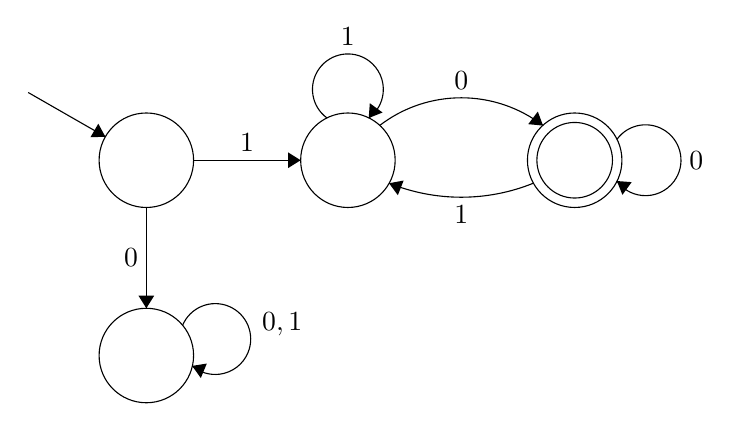
\begin{tikzpicture}[scale=0.2]
\tikzstyle{every node}+=[inner sep=0pt]
\draw [black] (24.1,-13.6) circle (3);
\draw [black] (24.1,-26) circle (3);
\draw [black] (36.9,-13.6) circle (3);
\draw [black] (51.3,-13.6) circle (3);
\draw [black] (51.3,-13.6) circle (2.4);
\draw [black] (38.912,-11.396) arc (127.51838:52.48162:8.518);
\fill [black] (49.29,-11.4) -- (48.96,-10.51) -- (48.35,-11.31);
\draw (44.1,-9.13) node [above] {$0$};
\draw [black] (48.685,-15.055) arc (-67.94171:-112.05829:12.209);
\fill [black] (39.51,-15.06) -- (40.07,-15.82) -- (40.44,-14.89);
\draw (44.1,-16.45) node [below] {$1$};
\draw [black] (53.98,-12.277) arc (144:-144:2.25);
\draw (58.55,-13.6) node [right] {$0$};
\fill [black] (53.98,-14.92) -- (54.33,-15.8) -- (54.92,-14.99);
\draw [black] (35.577,-10.92) arc (234:-54:2.25);
\draw (36.9,-6.35) node [above] {$1$};
\fill [black] (38.22,-10.92) -- (39.1,-10.57) -- (38.29,-9.98);
\draw [black] (27.1,-13.6) -- (33.9,-13.6);
\fill [black] (33.9,-13.6) -- (33.1,-13.1) -- (33.1,-14.1);
\draw (30.5,-13.1) node [above] {$1$};
\draw [black] (24.1,-16.6) -- (24.1,-23);
\fill [black] (24.1,-23) -- (24.6,-22.2) -- (23.6,-22.2);
\draw (23.6,-19.8) node [left] {$0$};
\draw [black] (16.6,-9.3) -- (21.5,-12.11);
\fill [black] (21.5,-12.11) -- (21.05,-11.28) -- (20.55,-12.14);
\draw [black] (26.399,-24.091) arc (157.4457:-130.5543:2.25);
\draw (31.42,-24.01) node [right] {$0,1$};
\fill [black] (27.01,-26.66) -- (27.56,-27.43) -- (27.94,-26.51);
\end{tikzpicture}
\end{center}



\item[16.A] Constructing equivalent DFA for the given NFA: 

1) $Q^1$ = p(Q) where $Q^1$ is the subset of all sets of Q. so $Q^1$ = ${\varnothing , (1), (2), (1,2) } $

2) $q^'$ $_0$ = ${q_0}$ where $q_0$ is the start state in NFA. here   $q^'$ $_0$ = {1}

3) $F^'$ = {$R \in Q^'$ |  $R$ contain an accept state of NFA} the machine M accepts the possible states where the NFA is present in the accept state. 

4) the state diagram for the equivalent DFA is as follows.



\begin{document}

\begin{center}
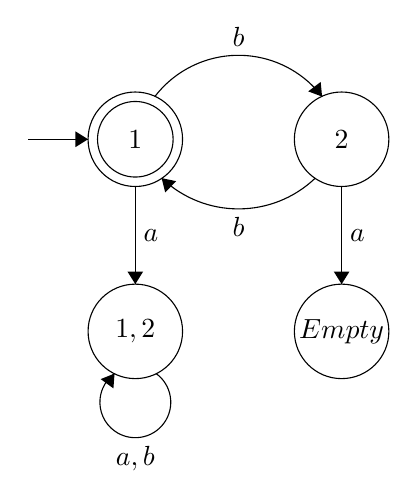
\begin{tikzpicture}[scale=0.2]
\tikzstyle{every node}+=[inner sep=0pt]
\draw [black] (35.4,-11) circle (3);
\draw (35.4,-11) node {$1$};
\draw [black] (35.4,-11) circle (2.4);
\draw [black] (48.5,-11) circle (3);
\draw (48.5,-11) node {$2$};
\draw [black] (35.4,-23.2) circle (3);
\draw (35.4,-23.2) node {$1,2$};
\draw [black] (48.5,-23.2) circle (3);
\draw (48.5,-23.2) node {$Empty$};
\draw [black] (36.637,-8.294) arc (142.58258:37.41742:6.69);
\fill [black] (47.26,-8.29) -- (47.17,-7.36) -- (46.38,-7.96);
\draw (41.95,-5.17) node [above] {$b$};
\draw [black] (46.83,-13.465) arc (-46.2822:-133.7178:7.061);
\fill [black] (37.07,-13.47) -- (37.3,-14.38) -- (37.99,-13.66);
\draw (41.95,-15.92) node [below] {$b$};
\draw [black] (35.4,-14) -- (35.4,-20.2);
\fill [black] (35.4,-20.2) -- (35.9,-19.4) -- (34.9,-19.4);
\draw (35.9,-17.1) node [right] {$a$};
\draw [black] (36.723,-25.88) arc (54:-234:2.25);
\draw (35.4,-30.45) node [below] {$a,b$};
\fill [black] (34.08,-25.88) -- (33.2,-26.23) -- (34.01,-26.82);
\draw [black] (48.5,-14) -- (48.5,-20.2);
\fill [black] (48.5,-20.2) -- (49,-19.4) -- (48,-19.4);
\draw (49,-17.1) node [right] {$a$};
\draw [black] (28.6,-11) -- (32.4,-11);
\fill [black] (32.4,-11) -- (31.6,-10.5) -- (31.6,-11.5);
\end{tikzpicture}
\end{center}


\item[28.A] Given regular expression $R = a(abb)*\cup b$
now we convert this regular expression into NFA by following steps

1)   NFA for A   

\begin{document}

\begin{center}
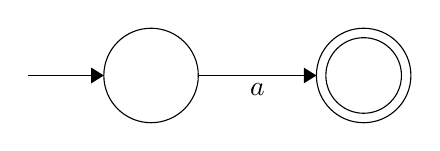
\begin{tikzpicture}[scale=0.2]
\tikzstyle{every node}+=[inner sep=0pt]
\draw [black] (25.5,-19.5) circle (3);
\draw [black] (39,-19.5) circle (3);
\draw [black] (39,-19.5) circle (2.4);
\draw [black] (28.5,-19.5) -- (36,-19.5);
\fill [black] (36,-19.5) -- (35.2,-19) -- (35.2,-20);
\draw (32.25,-20) node [below] {$a$};
\draw [black] (17.7,-19.5) -- (22.5,-19.5);
\fill [black] (22.5,-19.5) -- (21.7,-19) -- (21.7,-20);
\end{tikzpicture}
\end{center}

2)   NFA for B   

\begin{document}

\begin{center}
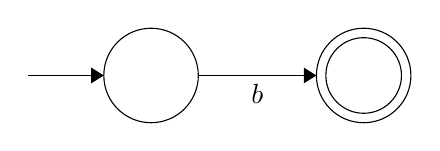
\begin{tikzpicture}[scale=0.2]
\tikzstyle{every node}+=[inner sep=0pt]
\draw [black] (25.5,-19.5) circle (3);
\draw [black] (39,-19.5) circle (3);
\draw [black] (39,-19.5) circle (2.4);
\draw [black] (28.5,-19.5) -- (36,-19.5);
\fill [black] (36,-19.5) -- (35.2,-19) -- (35.2,-20);
\draw (32.25,-20) node [below] {$b$};
\draw [black] (17.7,-19.5) -- (22.5,-19.5);
\fill [black] (22.5,-19.5) -- (21.7,-19) -- (21.7,-20);
\end{tikzpicture}
\end{center}

3)   NFA for (abb)*
\begin{document}

\begin{center}
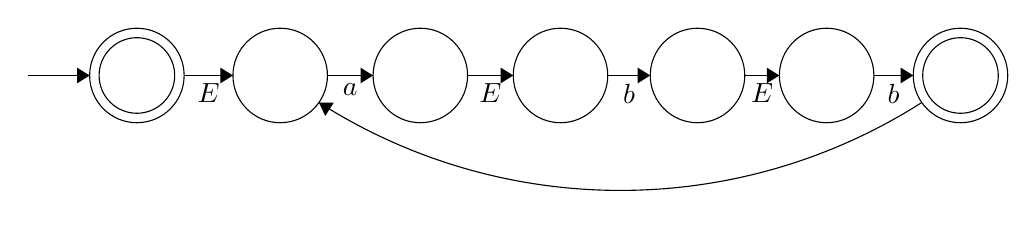
\begin{tikzpicture}[scale=0.2]
\tikzstyle{every node}+=[inner sep=0pt]
\draw [black] (9.7,-17.3) circle (3);
\draw [black] (9.7,-17.3) circle (2.4);
\draw [black] (18.8,-17.3) circle (3);
\draw [black] (27.7,-17.3) circle (3);
\draw [black] (36.6,-17.3) circle (3);
\draw [black] (45.3,-17.3) circle (3);
\draw [black] (53.5,-17.3) circle (3);
\draw [black] (62,-17.3) circle (3);
\draw [black] (62,-17.3) circle (2.4);
\draw [black] (2.8,-17.3) -- (6.7,-17.3);
\fill [black] (6.7,-17.3) -- (5.9,-16.8) -- (5.9,-17.8);
\draw [black] (12.7,-17.3) -- (15.8,-17.3);
\fill [black] (15.8,-17.3) -- (15,-16.8) -- (15,-17.8);
\draw (14.25,-17.8) node [below] {$E$};
\draw [black] (21.8,-17.3) -- (24.7,-17.3);
\fill [black] (24.7,-17.3) -- (23.9,-16.8) -- (23.9,-17.8);
\draw (23.25,-17.8) node [below] {$a$};
\draw [black] (30.7,-17.3) -- (33.6,-17.3);
\fill [black] (33.6,-17.3) -- (32.8,-16.8) -- (32.8,-17.8);
\draw (32.15,-17.8) node [below] {$E$};
\draw [black] (39.6,-17.3) -- (42.3,-17.3);
\fill [black] (42.3,-17.3) -- (41.5,-16.8) -- (41.5,-17.8);
\draw (40.95,-17.8) node [below] {$b$};
\draw [black] (48.3,-17.3) -- (50.5,-17.3);
\fill [black] (50.5,-17.3) -- (49.7,-16.8) -- (49.7,-17.8);
\draw (49.4,-17.8) node [below] {$E$};
\draw [black] (56.5,-17.3) -- (59,-17.3);
\fill [black] (59,-17.3) -- (58.2,-16.8) -- (58.2,-17.8);
\draw (57.75,-17.8) node [below] {$b$};
\draw [black] (59.541,-19.017) arc (-57.48076:-122.51924:35.606);
\fill [black] (21.26,-19.02) -- (21.66,-19.87) -- (22.2,-19.03);
\end{tikzpicture}
\end{center}



4)   NFA for a(abb*)\cup b 


\begin{document}

\begin{center}
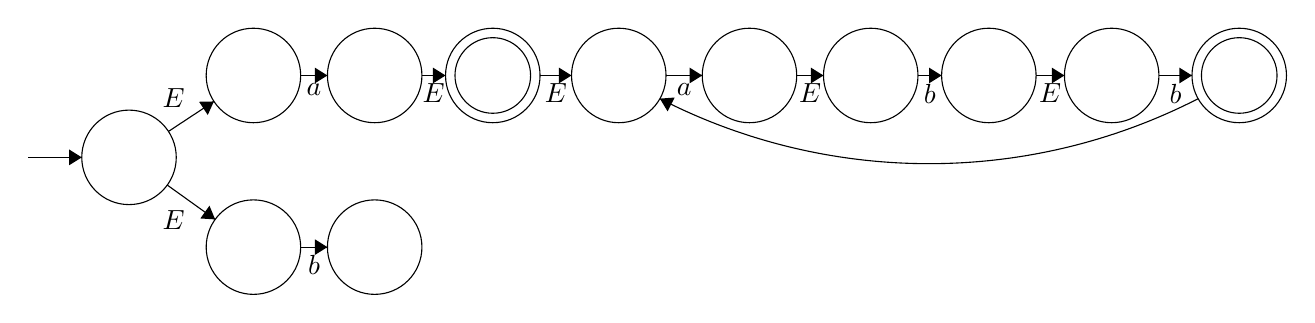
\begin{tikzpicture}[scale=0.2]
\tikzstyle{every node}+=[inner sep=0pt]
\draw [black] (29.4,-17.3) circle (3);
\draw [black] (29.4,-17.3) circle (2.4);
\draw [black] (37.4,-17.3) circle (3);
\draw [black] (45.7,-17.3) circle (3);
\draw [black] (53.4,-17.3) circle (3);
\draw [black] (60.9,-17.3) circle (3);
\draw [black] (68.7,-17.3) circle (3);
\draw [black] (76.8,-17.3) circle (3);
\draw [black] (76.8,-17.3) circle (2.4);
\draw [black] (21.9,-17.3) circle (3);
\draw [black] (14.2,-17.3) circle (3);
\draw [black] (6.3,-22.5) circle (3);
\draw [black] (14.2,-28.2) circle (3);
\draw [black] (21.9,-28.2) circle (3);
\draw [black] (32.4,-17.3) -- (34.4,-17.3);
\fill [black] (34.4,-17.3) -- (33.6,-16.8) -- (33.6,-17.8);
\draw (33.4,-17.8) node [below] {$E$};
\draw [black] (40.4,-17.3) -- (42.7,-17.3);
\fill [black] (42.7,-17.3) -- (41.9,-16.8) -- (41.9,-17.8);
\draw (41.55,-17.8) node [below] {$a$};
\draw [black] (48.7,-17.3) -- (50.4,-17.3);
\fill [black] (50.4,-17.3) -- (49.6,-16.8) -- (49.6,-17.8);
\draw (49.55,-17.8) node [below] {$E$};
\draw [black] (56.4,-17.3) -- (57.9,-17.3);
\fill [black] (57.9,-17.3) -- (57.1,-16.8) -- (57.1,-17.8);
\draw (57.15,-17.8) node [below] {$b$};
\draw [black] (63.9,-17.3) -- (65.7,-17.3);
\fill [black] (65.7,-17.3) -- (64.9,-16.8) -- (64.9,-17.8);
\draw (64.8,-17.8) node [below] {$E$};
\draw [black] (71.7,-17.3) -- (73.8,-17.3);
\fill [black] (73.8,-17.3) -- (73,-16.8) -- (73,-17.8);
\draw (72.75,-17.8) node [below] {$b$};
\draw [black] (74.188,-18.775) arc (-62.84258:-117.15742:37.439);
\fill [black] (40.01,-18.77) -- (40.5,-19.58) -- (40.95,-18.7);
\draw [black] (24.9,-17.3) -- (26.4,-17.3);
\fill [black] (26.4,-17.3) -- (25.6,-16.8) -- (25.6,-17.8);
\draw (25.65,-17.8) node [below] {$E$};
\draw [black] (17.2,-17.3) -- (18.9,-17.3);
\fill [black] (18.9,-17.3) -- (18.1,-16.8) -- (18.1,-17.8);
\draw (18.05,-17.8) node [below] {$a$};
\draw [black] (-0.1,-22.5) -- (3.3,-22.5);
\fill [black] (3.3,-22.5) -- (2.5,-22) -- (2.5,-23);
\draw [black] (8.81,-20.85) -- (11.69,-18.95);
\fill [black] (11.69,-18.95) -- (10.75,-18.97) -- (11.3,-19.81);
\draw (9.14,-19.4) node [above] {$E$};
\draw [black] (8.73,-24.26) -- (11.77,-26.44);
\fill [black] (11.77,-26.44) -- (11.41,-25.57) -- (10.83,-26.38);
\draw (9.14,-25.85) node [below] {$E$};
\draw [black] (17.2,-28.2) -- (18.9,-28.2);
\fill [black] (18.9,-28.2) -- (18.1,-27.7) -- (18.1,-28.7);
\draw (18.05,-28.7) node [below] {$b$};
\end{tikzpicture}
\end{center}








\item[29.B] Consider the language $A_2$ = {www|w \cup {a,b}*}

assume $A^2$ is a regular language. and let p be the pumping length given by the pumping lemma. 
By pumping lemma, this string can be divided into three pieces xyz such that |xy| < p, |y| > 0 and xy'z \cup $A^2$ > 0.

let aabaabaab be the string that belongs to $A^2$. the pumping length of the string is 2. to satisfy the conditions of the pumping lemma, x = a, y = a, z = baabaab. so S = aabaabaab = $(\frac{a}{x})$  $(\frac{a}{y})$ $(\frac{baabaab}{z})$

pump the middle part such that xy'z (i>0). for i = 2 the y becomes aa. the string after pumping is aaabaabaab. so S = (a) (a)' (baabaab) = $\frac{a}{x}$ $\frac{aa}{y}$ $\frac{baabaab}{z}$


the string aaabaabaab is not element of $A_2$ it is a contradiction. so the pumping lemma is violed therefore $A^2$ is not a regular language.




\item[60] $C_k$ is the language consisting of all strings that contains an a exactly k places from the right hand end. let N be the NFA with K+1 states that recognizes $C_k$
1) the state diagram of NFA N is followsL


\begin{document}

\begin{center}
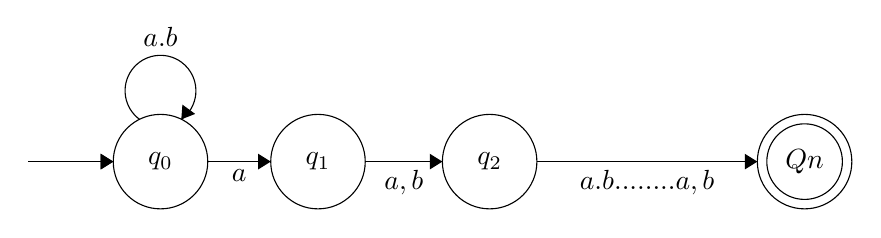
\begin{tikzpicture}[scale=0.2]
\tikzstyle{every node}+=[inner sep=0pt]
\draw [black] (11.2,-16.7) circle (3);
\draw (11.2,-16.7) node {$q_0$};
\draw [black] (21.2,-16.7) circle (3);
\draw (21.2,-16.7) node {$q_1$};
\draw [black] (32.1,-16.7) circle (3);
\draw (32.1,-16.7) node {$q_2$};
\draw [black] (52.1,-16.7) circle (3);
\draw (52.1,-16.7) node {$Qn$};
\draw [black] (52.1,-16.7) circle (2.4);
\draw [black] (14.2,-16.7) -- (18.2,-16.7);
\fill [black] (18.2,-16.7) -- (17.4,-16.2) -- (17.4,-17.2);
\draw (16.2,-17.2) node [below] {$a$};
\draw [black] (24.2,-16.7) -- (29.1,-16.7);
\fill [black] (29.1,-16.7) -- (28.3,-16.2) -- (28.3,-17.2);
\draw (26.65,-17.2) node [below] {$a,b$};
\draw [black] (35.1,-16.7) -- (49.1,-16.7);
\fill [black] (49.1,-16.7) -- (48.3,-16.2) -- (48.3,-17.2);
\draw (42.1,-17.2) node [below] {$a.b........a,b$};
\draw [black] (8.2,-16.7) -- (8.2,-16.7);
\fill [black] (8.2,-16.7) -- (7.4,-16.2) -- (7.4,-17.2);
\draw [black] (9.877,-14.02) arc (234:-54:2.25);
\draw (11.2,-9.45) node [above] {$a.b$};
\fill [black] (12.52,-14.02) -- (13.4,-13.67) -- (12.59,-13.08);
\draw [black] (2.8,-16.7) -- (8.2,-16.7);
\fill [black] (8.2,-16.7) -- (7.4,-16.2) -- (7.4,-17.2);
\end{tikzpicture}
\end{center}


2) the formal description of NFA 

Similar to a DFA, the formal definition of NFA is: (Q, E, δ, $q_0$, F), where

Q is a finite set of all states

E is a finite set of all symbols of the alphabet

δ: Q x E→ Q is the transition function from state to state

$q_0$ ∈ Q is the start state, in which the start state must be in the set Q

F ⊆ Q is the set of accept states, in which the accept states must be in the set Q

\end{document}
\end{document}
\end{document}
\end{document}
\end{document}
\end{document}
\end{document}
\end{document}
\end{document}
\end{document} 
\end{document} 
\end{itemize}
\end{document}